
\begingroup

\thispagestyle{empty} % Sem Cabeçalho e Rodapé

\begin{tikzpicture}[remember picture,overlay]

\node[inner sep=0pt] (background) at (current page.center) {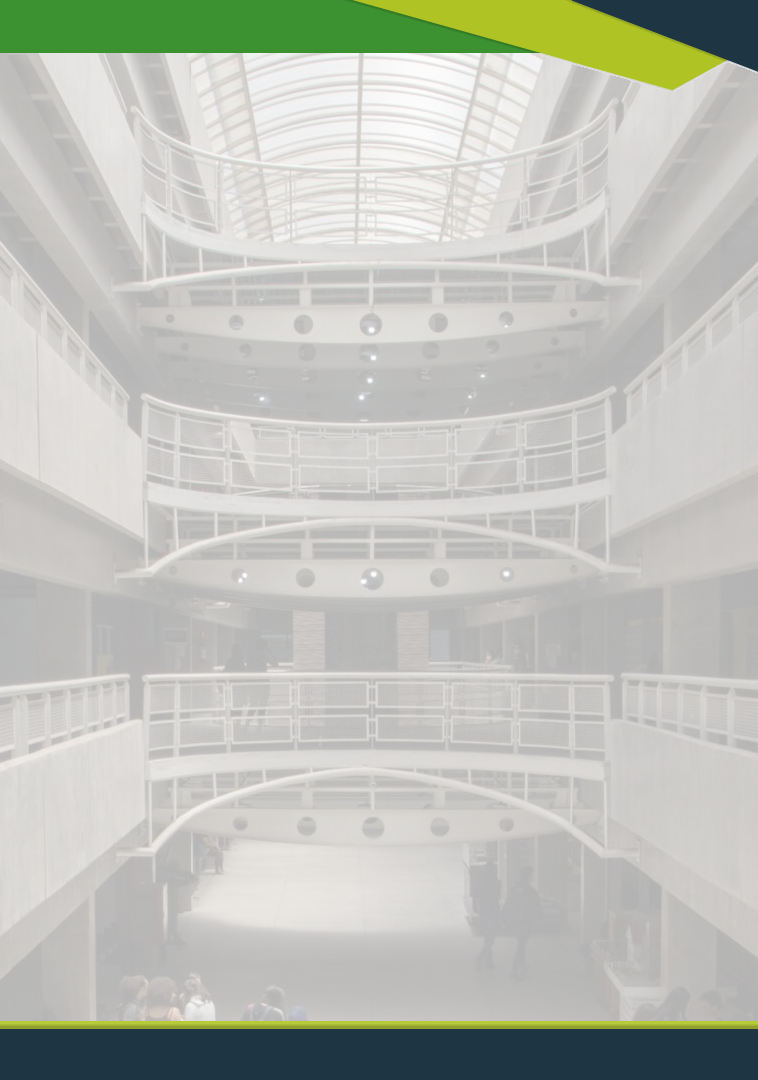
\includegraphics[width=\paperwidth]{Pictures/background.png}};
\draw (current page.center) node [fill=ocre,text opacity=1,inner sep=1cm]{\color{chapterhead}\Huge\centering\bfseries\sffamily\parbox[c][][t]{\paperwidth}{\centering \namesubject\\[15pt] % Nome da Matéria
{\Large \namecycle}%%Período do ciclo
}};

\end{tikzpicture}

\vfill
\Large\centering\text\sffamily{\centering\color{ocre}\nameauthor}

\Large\centering\text\sffamily{\centering\color{ocre}{\namecourse}}%curso

\Large\centering\bfseries\sffamily{\centering\color{ocre}{\nameinstitute}}%Instituição

\endgroup



